\documentclass[12pt]{article}
\usepackage{fullpage}
\usepackage{amsmath}
\usepackage{graphicx}
\usepackage{geometry}
\usepackage{sidecap}

\author{Pieter Vermeesch\\ {\tt cosmocalc@gmail.com}}
\title{CosmoCalc manual}
\date{}

\begin{document}

\maketitle

\begin{minipage}[tbp]{\textwidth}
{\tt CosmoCalc.xla}  is an Excel add-in designed  with the intention
  to  implement the  increasingly sophisticated  tools  of terrestrial
  cosmogenic  nuclide  geochronology  in  a user-friendly  way,  while
  enforcing the good practice of  using a consistent set of production
  rate scaling factors for both  the calibration sites and the unknown
  samples.  The add-in as  well as the {\tt CosmoTest.xls} spreadsheet
  with test  data can  be downloaded from  the CosmoCalc  website {\tt
    http://cosmocalc.london-geochron.com}.    Full   details   about   the
  calculations    are     provided    in    the     G-Cubed    article
  \cite{vermeesch2007}.\\

\begin{tabular}{lp{8cm}}
  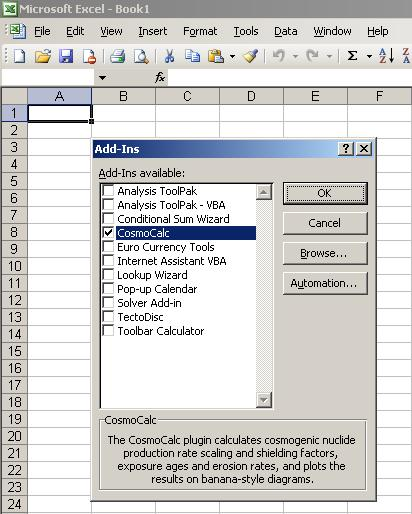
\includegraphics[width=.4\textwidth]{checkedAddIn.jpg}
& \vspace{-3.8cm}
  CosmoCalc can be installed by downloading  \texttt{CosmoCalc.xla}  
  to  the  Excel Add-Ins  folder.  Start  Excel and  select
  Tools $\rightarrow$ Add-Ins, or More Commands $\rightarrow$ Add-Ins
in Excel2010 and above. An Add-In is enabled when its checkbox
  is  marked.  The  Add-In  is  disabled by  unmarking  the  CosmoCalc
  checkbox. To remove the program, simply remove the .xla file from the
  Add-In folder.}
\end{tabular}
\end{minipage}


\begin{minipage}[tbp]{\textwidth}
  \begin{center}
  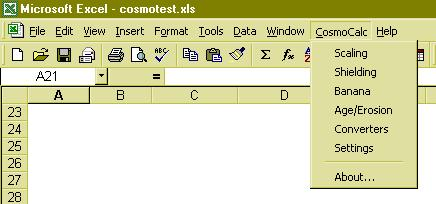
\includegraphics[width=.6\textwidth]{menu.jpg}\\
  \end{center}
  After  installing  the  add-in  (see downloadable  instructions),  a
  toolbar menu appears that guides the user through the data reduction
  and closely follows the outline  of this manual. The following pages
  will show how to scale  production rates for latitude and elevation,
  how  to  calculate  topographic,  snow and  self-shielding  factors,
  generate  banana-plots,  calculate exposure  ages,  burial ages  and
  erosion   rates,  and   calculate  geomagnetic   cutoff  rigidities,
  atmospheric depths and so forth.
  \\
\end{minipage}

\begin{minipage}[tbp]{\textwidth}
\begin{center}
  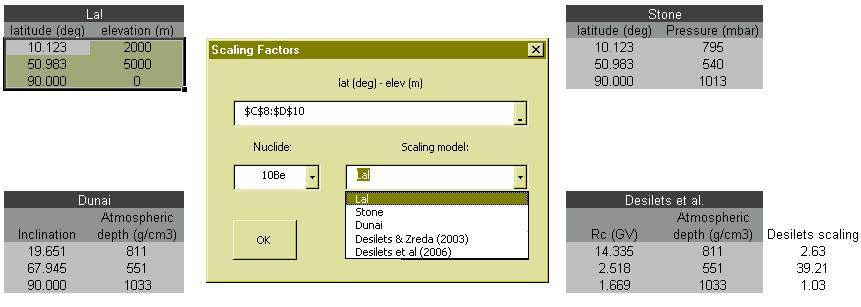
\includegraphics[width=\textwidth]{scaling.jpg}\\
\end{center}
  Cosmogenic  nuclide production  rates  are a  sensitive function  of
  latitude  and elevation,  and a  lively debate  is going  on  in the
  community  as  to how  to  best  calculate  these scaling  factors.  
  CosmoCalc   presently   implements    four   scaling   models:   Lal
  \cite{lal1991},  Stone \cite{stone2000}, Dunai  \cite{dunai2000} and
  Desilets \cite{desilets2003}\cite{desilets2006}.  Although the more
  recent models such as those  by Dunai and Desilets are significantly
  more sophisticated  than the  early scaling model  by Lal,  they are
  just as  easy to use  in CosmoCalc: just  select two columns  with a
  measure of  the sample's latitude and elevation,  select the nuclide
  and scaling model of interest and click ``OK''.
  \\
\end{minipage}

\begin{minipage}[tbp]{\textwidth}
\begin{center}
  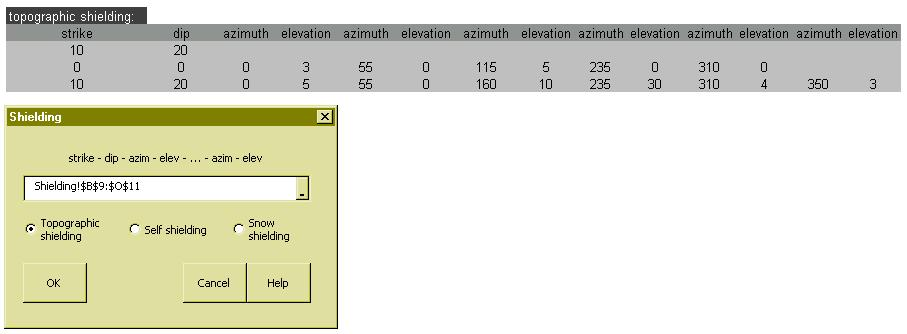
\includegraphics[width=.71\textwidth]{shieldingTopo.jpg}\\
  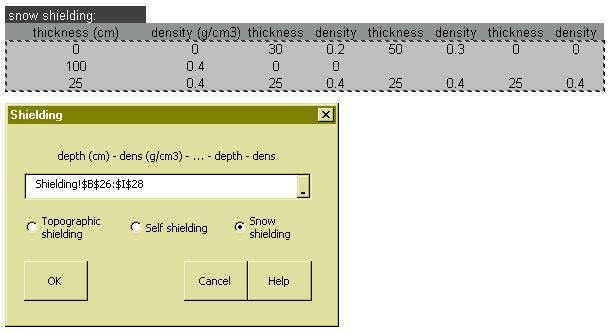
\includegraphics[width=.6\textwidth]{shieldingSnow.jpg}
  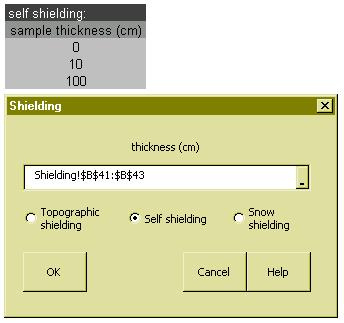
\includegraphics[width=.35\textwidth]{shieldingSelf.jpg}\\
\end{center}
  It is equally simple to compute topographic, snow and self-shielding
  factors. The  nuclide concentrations and the product  of the scaling
  and shielding  factors are the  only input required for  all further
  calculations.
  \\
\end{minipage}

CosmoCalc   uses  the   ingrowth   equation  of   Granger  and   Smith
\cite{granger2000}, which is a summation of four exponentials: one for
neutrons, two for slow muons and one for fast muons.

$$N(t,\epsilon,\tau) = P e^{- \lambda \tau}
\sum_{i=0}^3
\frac{S_i F_i}{\lambda + \epsilon \rho / \Lambda_i} 
\left( 1 - e^{- \left( \lambda + \epsilon \rho / \Lambda_i \right) t} \right)
$$

with:\\

\begin{center}
  \begin{tabular}{ll}
N = nuclide concentration & t = age\\
$\epsilon$ = erosion rate & $\tau$ = burial age \\
P = SLHL production rate & $\rho$ = rock density\\
$\lambda$ = decay constant & $\Lambda_i$ = attenuation length \\
S$_i$ = scaling factor & F$_i$ = relative production\\
i = 0: neutrons & i = 1, 2: slow muons\\
i = 3: fast muons & ~\\
\end{tabular}\\
\end{center}

Default values for  the various parameters in this  equation are those
advocated by  \cite{granger2000}, but  alternative values can  also be
set.    In  a   simple  exposure   history,  the   cosmogenic  nuclide
concentration is a function of  the exposure age, the erosion rate and
the burial  age.  Those are three  parameters, so if  only one nuclide
was measured,  we need two  assumptions, whereas if two  nuclides were
analysed, of which  at least one radionuclide, only  one assumption is
needed.
\\

\begin{minipage}[tbp]{\textwidth}
  \begin{center}
  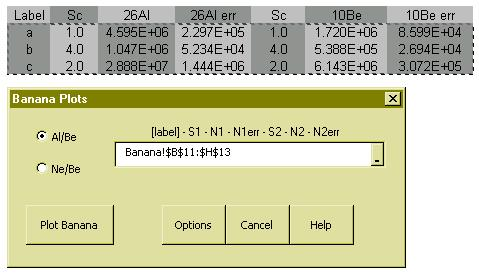
\includegraphics[width=.6\textwidth]{AlBeBanana.jpg}\\
  \end{center}
  Measuring two  nuclides also allows the generation  of banana-plots. 
  These are  sophisticated devices which  depend on a large  number of
  parameters,  such as  the production  rates  at sea  level and  high
  latitude,  the scaling model,  and the  relative proportions  of the
  various production mechanisms. Prior to CosmoCalc, banana plots were
  often    generated     in    graphics    applications     such    as
  Grapher$^\copyright$.  The advantage of  CosmoCalc is once again its
  flexibility.   Different  kinds of  Al-Be  and  Ne-Be  plots can  be
  generated on the fly.
  \\
\end{minipage}

\begin{minipage}[tbp]{\textwidth}
\begin{center}
  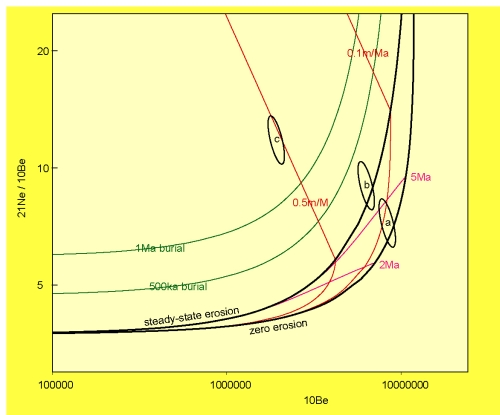
\includegraphics[width=.49\textwidth]{NeBeBananaWithoutMuonsSmall.jpg}
  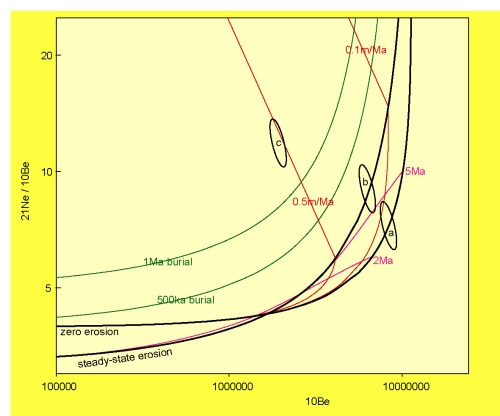
\includegraphics[width=.49\textwidth]{NeBeBananaWithMuonsSmall.jpg}\\
\end{center}
  These two  Ne-Be plots,  for example, show  how the  contribution of
  muons  causes a characteristic  cross-over between  the steady-state
  and zero erosion lines, which is absent when muons are neglected.
  \\
\end{minipage}

\begin{minipage}[tbp]{\textwidth}
  \begin{center}
  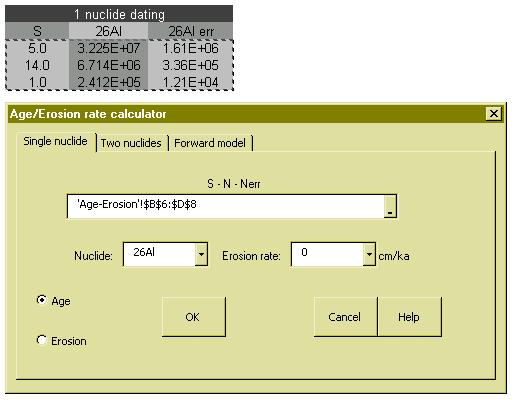
\includegraphics[width=.6\textwidth]{singleNuclideAge.jpg}\\
  \end{center}
  Given a  scaling factor and  the concentration of a  single nuclide,
  and assuming  zero burial, CosmoCalc  can either calculate  a steady
  state erosion rate, or a finite exposure age under the assumption of
  a particular erosion rate.
  \\
\end{minipage}

Only  one assumption  is needed  if  two nuclides  were measured.  For
example, by assuming an erosional steady state and setting an infinite
exposure age,  CosmoCalc simultaneously computes the  erosion rate and
burial age:

$$
\left\{
\begin{array}{l}
f_1(\epsilon,\tau): N_1 = P_1 e^{- \lambda_1 \tau} \sum_{i=0}^3 
   \frac{S_{i,1} F_{i,1}}{\lambda_1 + \epsilon \rho / \Lambda_{i,1}}\\
f_2(\epsilon,\tau): N_2 = P_2 e^{- \lambda_2 \tau} \sum_{i=0}^3 
   \frac{S_{i,2} F_{i,2}}{\lambda_2 + \epsilon \rho / \Lambda_{i,2}}
\end{array}\right.
$$

Alternatively,  if a  sample plots  inside the  erosion island  of the
banana  plot, we  can safely  assume zero  burial,  and simultaneously
compute the exposure age and erosion rate:

$$
\left\{
\begin{array}{l}
f_1(\epsilon,t):  N_1 = P_1 \sum_{i=0}^3\frac{S_{i,1} F_{i,1}}{\lambda_1 + \epsilon \rho / \Lambda_{i,1}} 
    \left( 1 - e^{- \left( \lambda_1 + \epsilon \rho / \Lambda_{i,1} \right) t} \right)\\
f_2(\epsilon,t):  N_2 = P_2 \sum_{i=0}^3\frac{S_{i,2} F_{i,2}}{\lambda_2 + \epsilon \rho / \Lambda_{i,2}} 
    \left( 1 - e^{- \left( \lambda_2 + \epsilon \rho / \Lambda_{i,2} \right) t} \right)
\end{array}\right.
$$

\begin{minipage}[tbp]{\textwidth}
  \begin{center}
  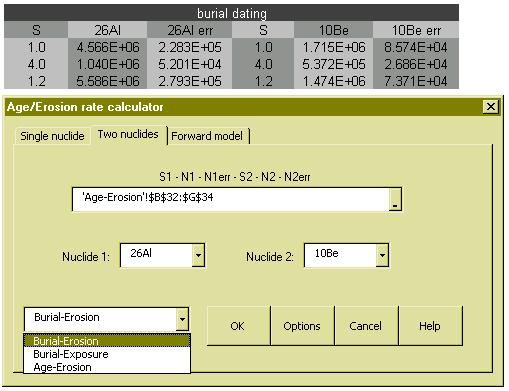
\includegraphics[width=.6\textwidth]{twoNuclideAge.jpg}\\
  \end{center}
  All  these calculations  are  equally simple  in CosmoCalc.   Simply
  select the  desired calculation and the two  nuclides from pull-down
  menus, select  two times three  columns of the spreadsheet  with the
  correction factors, the  nuclide concentrations and their 1-$\sigma$
  uncertainties, and click ``OK''.
  \\
\end{minipage}

\begin{minipage}[tbp]{\textwidth}
  \begin{center}
  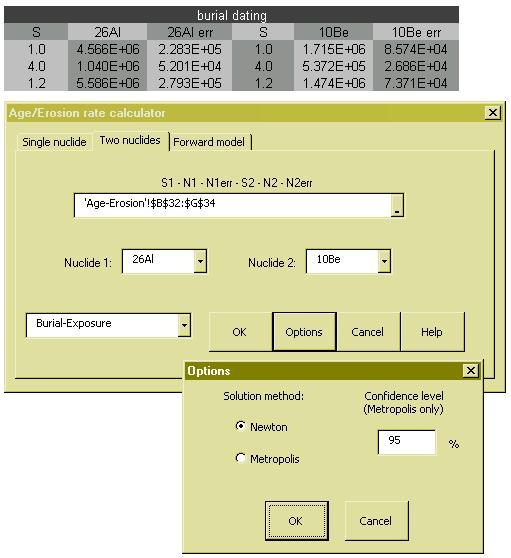
\includegraphics[width=.6\textwidth]{twoNuclideOptions.jpg}\\
  \end{center}
  CosmoCalc   implements  two  numerical   techniques  to   solve  the
  non-linear systems  of equations.   The default is  Newton's method,
  which is a very fast  and exact algorithm.  The Metropolis algorithm
  is offered as an alternative.
  \\
\end{minipage}

\begin{minipage}[tbp]{\textwidth}
\begin{center}
  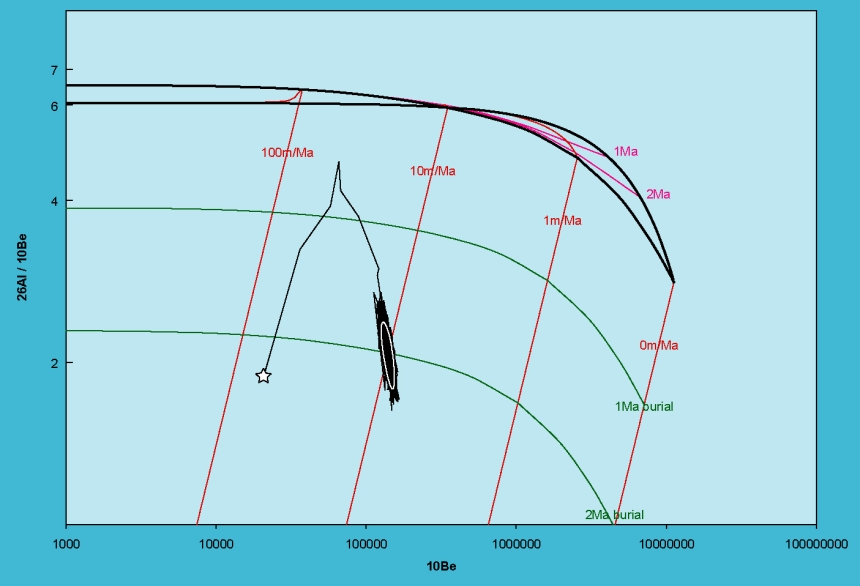
\includegraphics[width=\textwidth]{metropolisBananaSmall.jpg}\\
\end{center}
  The  Metropolis   algorithm  is  a   Monte  Carlo  method   that  is
  computationally  considerably more intensive  than Newton's  method. 
  Over a thousand iterations, it first converges from an initial guess
  to  the correct  solution and  then continues  to sample  the entire
  solution  space.  The  Metropolis  algorithm has  two advantages  of
  Newton's method. First, it will  always find a solution, even if the
  sample  plots just  into  the so-called  ``forbidden  zone'' of  the
  banana plot. Newton's method would diverge in this case.
  \\
\end{minipage}

\begin{minipage}[tbp]{\textwidth}
Second, the Metropolis algorithm will yield asymmetric and therefore more meaningful
confidence intervals than the symmetric confidence bounds given by Newton's method, which
are calculated by standard error propagation.\\
Newton:\\
   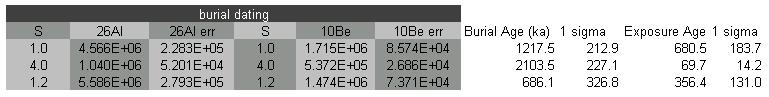
\includegraphics[width = .9\textwidth]{twoNuclideNewtonResults.jpg}\\
Metropolis:\\
   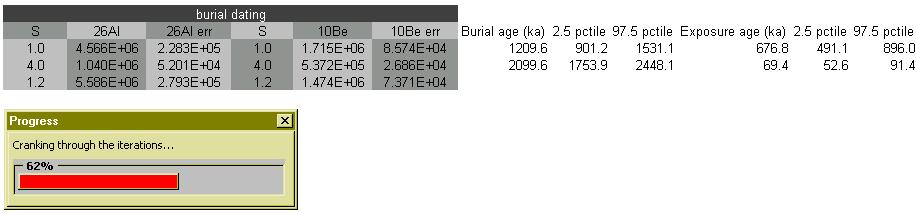
\includegraphics[width = \textwidth]{twoNuclideMetropolisResults.jpg}
\end{minipage}

\begin{minipage}[tbp]{\textwidth}
  \begin{center}
  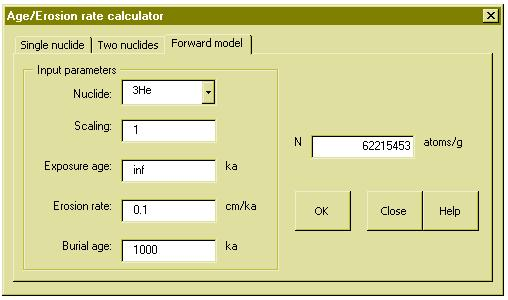
\includegraphics[width=.6\textwidth]{forward.jpg}\\
  \end{center}
  CosmoCalc  also provides  a useful  forward modeling  function. This
  function was  used to generate  the synthetic data of  the CosmoTest
  worksheet.
  \\
\end{minipage}

\begin{minipage}[tbp]{\textwidth}
\begin{center}
  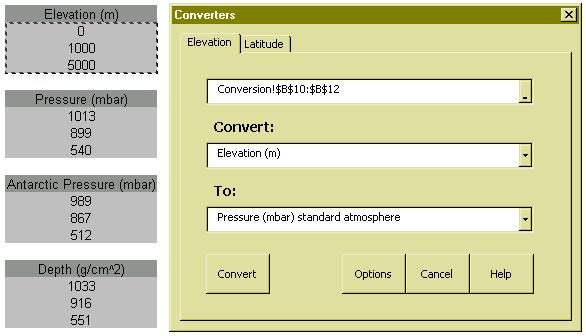
\includegraphics[width=.49\textwidth]{converterElev.jpg}
  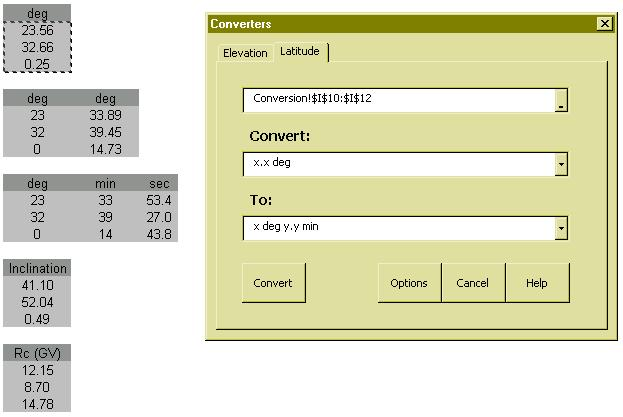
\includegraphics[width=.5\textwidth]{converterLat.jpg}\\
\end{center}
  Different scaling  models use different  kinds of geographic  input. 
  For example,  Lal's scaling model uses elevation  whereas Stone uses
  atmospheric  pressure  and Dunai  and  Desilets  atmospheric depth.  
  Furthermore, Lal  and Stone  use geomagnetic latitude  whereas Dunai
  uses  geomagnetic  inclination  and  Desilets cutoff  rigidity.   To
  facilitate the  comparison of the various  scaling models, CosmoCalc
  provides some easy-to-use conversion tools.
  \\
\end{minipage}

\begin{minipage}[tbp]{\textwidth}
  \begin{center}
  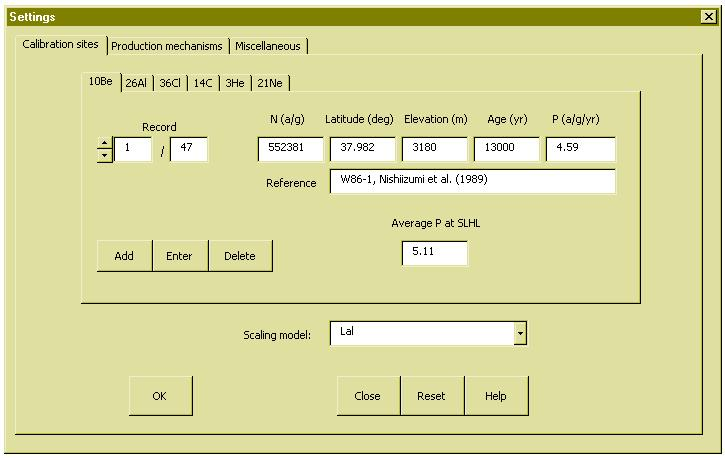
\includegraphics[width=.65\textwidth]{settingsCalSites.jpg}\\
  \end{center}
  Scaling factors are  the subject of much debate,  and are definitely
  an important  issue, but they all  have one thing  in common, namely
  the  crucial importance  of using  the  same scaling  model for  the
  unknown  sample  and  the   calibration  sites.   For  this  reason,
  CosmoCalc  defines  the production  rates  not  explicitly but  {\it
    implicitly}, by specifying the raw measurements of the calibration
  sites.  The program  comes with a set of  default calibration sites,
  but this list can be modified by removing and adding new sites.
  \\
\end{minipage}

\begin{minipage}[tbp]{\textwidth}
  \begin{center}
  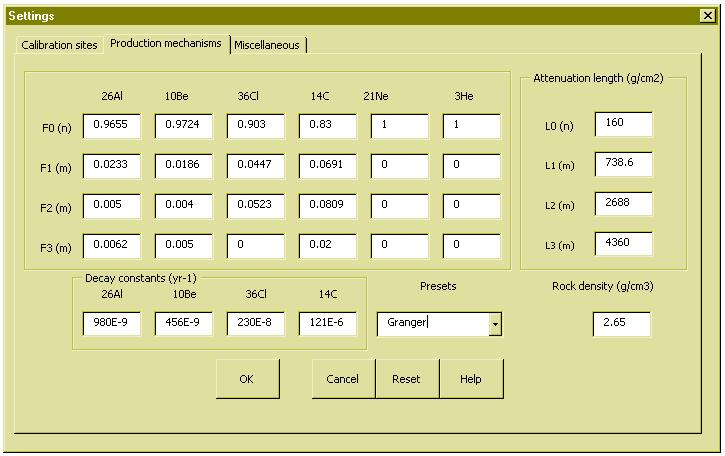
\includegraphics[width=.65\textwidth]{settingsProdMech.jpg}\\
  \end{center}
  It was  shown earlier  that the  ingrowth equation is  made up  of 4
  exponentials,  all parameters  of which  can be  customized  in this
  menu, where the relative contribution  of neutrons and muons as well
  as  their respective attenuation  lengths can  be set.   The default
  values    are    those   recommended    by    Granger   and    Smith
  \cite{granger2000},  but  alternative  options  are also  given,  or
  custom values  can be  set by the  user.  For example,  the ingrowth
  equation of Schaller et  al. \cite{schaller2002}, which contains not
  4 but 8 exponentials, is implemented in CosmoCalc by a least squares
  approximation of four exponentials.
  \\
\end{minipage}

\begin{minipage}[tbp]{\textwidth}
  \begin{center}
   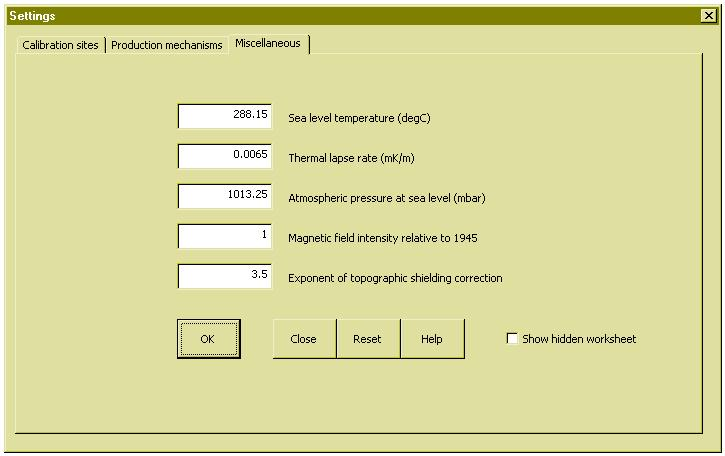
\includegraphics[width=.65\textwidth]{settingsMisc.jpg}\\
  \end{center}
  Finally,  some leftover  parameters  important for  the scaling  and
  shielding factors can be set on  the last tab of the shielding menu.
\\
\end{minipage}

\begin{thebibliography}{}

\bibitem{vermeesch2007}  Vermeesch,  P.,  2007,  CosmoCalc:  an  Excel
  add-in   for    cosmogenic   nuclide   calculations:   Geochemistry,
  Geophysics, and Geosystems (in press)
  
\bibitem{lal1991} Lal, D., Cosmic ray labeling of erosion surfaces: in
  situ  nuclide production rates  and erosion  models, {\it  Earth and
    Planetary Science Letters, 104}, 424-439, 1991.
  
\bibitem{stone2000}  Stone, J.,  Air pressure  and  cosmogenic isotope
  production, {\it Journal of Geophysical Research, 105}, 23753-23759,
  2000.
  
\bibitem{dunai2000} Dunai, T.J.,  Scaling factors for production rates
  of in  situ produced  cosmogenic nuclides: a  critical reevaluation,
  {\it Earth and Planetary Science Letters, 176}, 157-169, 2000.
  
\bibitem{desilets2003}  Desilets,  D.,   and  M.  Zreda,  Spatial  and
  temporal  distribution of  secondary cosmic-ray  nucleon intensities
  and  applications  to in  situ  cosmogenic  dating,  {\it Earth  and
    Planetary Science Letters, 206}, 21-42, 2003.
  
\bibitem{desilets2006} Desilets, D., M.  Zreda, and T. Prabu, Extended
  scaling factors for in situ cosmogenic nuclides: New measurements at
  low  latitude,  {\it  Earth  and Planetary  Science  Letters,  246},
  265-276, 2006.
  
\bibitem{granger2000}  Granger, D.E.,  and A.L.  Smith,  Dating buried
  sediments  using  radioactive   decay  and  muogenic  production  of
  $^{26}$Al  and $^{10}$Be,  {\it Nuclear  Instruments and  Methods in
    Physics Research B, 172}, 822-826, 2000.
  
\bibitem{schaller2002} Schaller, M., F. von Blanckenburg, A. Veldkamp,
  L.A.  Tebbens, N.   Hovius, and  P.W.   Kubik, A  30000yr record  of
  erosion  rates  from cosmogenic  $^{10}$Be  in  Middle Europe  river
  terraces, {\it  Earth and Planetary Science  Letters, 204}, 307-320,
  2002.

\end{thebibliography}

\end{document}
